% Phụ lục: số liệu chi tiết và phương pháp của Chương 2 (đề cho phép: phụ lục không tính vào giới hạn 10–15 trang).
% Bảng do scripts/make_figures.jl sinh vào tables/, riêng Bảng R_tree viết tay từ results/fptree/fptree_size.csv.

% Phụ lục bắt đầu ở trang mới (\clearpage đẩy hết hình, bảng còn chờ của các chương ra trước).
\clearpage
\pdfbookmark[0]{Phụ lục}{appendix}
\appendices
\section{Số liệu chi tiết của Chương 2}
\label{app:tables}

Các bảng và hình dưới đây là số liệu chi tiết cho các hình trong Chương~\ref{sec:experiments}. Trong
Bảng~\ref{tab:ratio}, M1..M7 là các mức minsup của từng CSDL theo thứ tự từ cao xuống thấp như trong
\path{data/meta/benchmark_config.csv}, ví dụ chess là 90, 85, \ldots, 60\%.

\begin{table}[H]
\caption{Tỉ lệ thời gian nhóm/SPMF, M1..M7 là các mức minsup từ cao xuống thấp}
\label{tab:ratio}
\centering
\fittable{\columnwidth}{runtime_ratio_table}
\end{table}

\begin{table*}[!t]
\caption{Phân rã thời gian (giây) của nhóm ở minsup thấp nhất: đọc file, khai thác, ghi file, so với SPMF}
\label{tab:breakdown}
\centering
\fittable{\textwidth}{runtime_breakdown_table}
\end{table*}

\textbf{Phân rã thời gian.} Ba thành phần đọc, khai thác, ghi trong Bảng~\ref{tab:breakdown} lấy từ cùng lần đo có
tổng thời gian là trung vị, nên tổng chỉ lệch do làm tròn. Bước khai thác gồm cả dựng FP-tree. Cột cuối là thời gian khai thác của nhóm chia cho
\emph{tổng} thời gian của SPMF. Hai số không cùng phạm vi, nên cột này chỉ là chỉ số chẩn đoán: giá trị lớn hơn 1 cho
biết riêng bước khai thác của nhóm đã lâu hơn toàn bộ thời gian chạy của SPMF, không cho biết tỉ lệ giữa hai bước
khai thác.

\textbf{Tỉ lệ kích thước FP-tree.} Mức chia sẻ tiền tố được đo bằng
\begin{equation}
R_{\text{tree}}=\frac{N_{\text{nodes}}}{\sum_{i=1}^{n}|T'_i|}\times 100\%,
\label{eq:tree-ratio}
\end{equation}
với $N_{\text{nodes}}$ là số nút của FP-tree gốc (không tính nút gốc) và $T'_i$ là giao dịch thứ $i$ sau khi bỏ các
item không phổ biến. Mẫu số là số nút tối đa khi không giao dịch nào chung tiền tố, nên $R_{\text{tree}}$ càng nhỏ thì
cây nén càng tốt. Đây là tỉ lệ số nút, không phải tỉ lệ bộ nhớ (Bảng~\ref{tab:fptree}).

% Số liệu từ results/fptree/fptree_size.csv (scripts/fptree_size.jl), minsup giữa lưới của mỗi CSDL.
\begin{table}[H]
\caption{Tỉ lệ kích thước FP-tree gốc $R_{\text{tree}}$ ở minsup giữa lưới}
\label{tab:fptree}
\centering
\footnotesize\setlength{\tabcolsep}{3.5pt}
\begin{tabular}{llrrrr}
\hline
Dataset & Loại & minsup (\%) & \begin{tabular}[b]{@{}c@{}}Item\\phổ biến\end{tabular} & Số nút & $R_{\text{tree}}$ (\%) \\
\hline
chess & dày & 75 & 23 & 1\,898 & 2,85 \\
mushrooms & dày & 7 & 64 & 18\,658 & 10,56 \\
connect & dày & 85 & 25 & 411 & 0,03 \\
pumsb\_star & dày & 50 & 27 & 18\,766 & 2,24 \\
accidents & dày & 70 & 16 & 5\,070 & 0,11 \\
retail & thưa & 0,2 & 956 & 292\,501 & 56,08 \\
T10I4D100K & thưa & 0,2 & 741 & 703\,357 & 70,47 \\
T40I10D100K & thưa & 2 & 610 & 3\,259\,405 & 89,13 \\
kosarak & thưa & 0,4 & 212 & 1\,087\,185 & 28,14 \\
\hline
\end{tabular}
\end{table}

\begin{table}[H]
\caption{Bộ nhớ và thời gian khai thác của ba biến thể basic, paper, optimized (trung vị 3 lần đo)}
\label{tab:memory}
\centering
\fittable{\columnwidth}{memory_table}
\end{table}

\begin{table*}[!t]
\caption{Ablation: thời gian khai thác của từng biến thể chia cho bản optimized (lớn hơn 1: chậm hơn bản optimized)}
\label{tab:ablation}
\centering
\fittable{\textwidth}{ablation_table}
\end{table*}

\begin{table}[H]
\caption{Thời gian (giây) trên các tập con của retail}
\label{tab:scalability}
\centering
\fittable{\columnwidth}{scalability_table}
\end{table}

\begin{figure*}[!t]
\centering
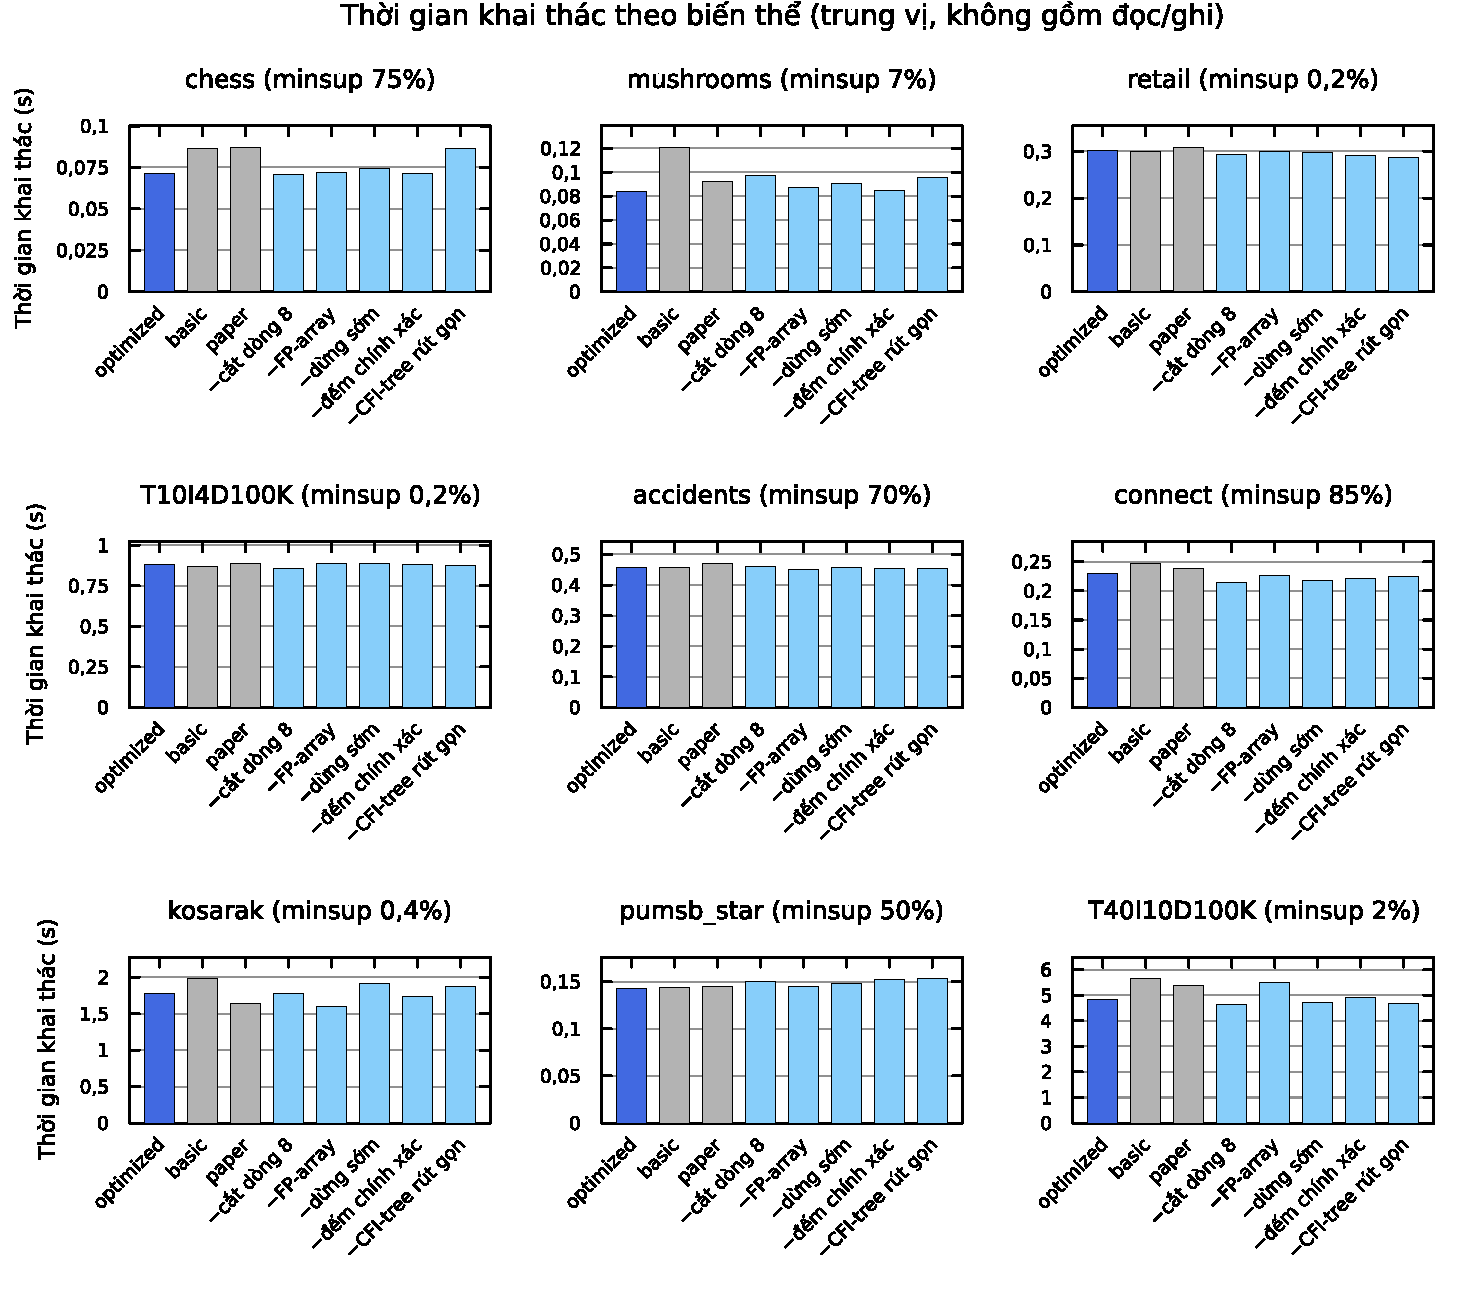
\includegraphics[width=0.82\textwidth]{time_variants_grid.pdf}
\caption{Thời gian khai thác của tám biến thể tại minsup giữa lưới (trung vị 3 lần đo, không gồm đọc và ghi file).}
\label{fig:time-variants}
\end{figure*}

\begin{table}[H]
\caption{Số tập đóng và thời gian (giây) theo độ dài giao dịch trung bình}
\label{tab:txlen}
\centering
\fittable{\columnwidth}{txlen_table}
\end{table}

% Đẩy hết bảng còn chờ của Phụ lục A (kể cả bảng rộng hai cột) ra trước khi sang Phụ lục B
\clearpage
\section{Dữ liệu và phương pháp đo}
\label{app:data}

\textbf{Chuẩn hóa dữ liệu.} Hai CSDL FIMI có mã item bắt đầu từ 0 (pumsb\_star và T40I10D100K) được ánh xạ mỗi item
$i$ thành $f(i)=i+1$. Phép ánh xạ một-một này bảo toàn nội dung giao dịch, support và tính đóng của các itemset
($\operatorname{supp}_D(X)=\operatorname{supp}_{f(D)}(f(X))$), nên sau chuẩn hóa cả chín CSDL chỉ chứa item có mã
nguyên dương. Quá trình chuẩn hóa chỉ thay đổi cách biểu diễn, không loại bỏ các giao dịch trùng nội dung, nhằm bảo
toàn support của các itemset.

\textbf{Phiên bản mushrooms.} Bản SPMF có 8\,416 giao dịch nhưng chỉ 8\,124 giao dịch phân biệt về nội dung, tương
ứng 292 lượt giao dịch lặp. Bản FIMI có đúng 8\,124 giao dịch, bằng số mẫu của UCI Mushroom~\cite{uci_mushroom}. Do
hai bản mã hóa item khác nhau, nhóm thống nhất dùng bản FIMI cho toàn bộ thực nghiệm.

\textbf{Độ biến thiên.} Mức biến thiên giữa 3 lần đo của mỗi cấu hình được tính bằng khoảng biến thiên tương đối
(\textit{relative range})
\begin{equation}
V=\frac{T_{\max}-T_{\min}}{T_{\min}}\times 100\%.
\label{eq:relrange}
\end{equation}
Trên 56 cấu hình minsup, trung vị của $V$ là 5{,}2\% với nhóm và 4{,}5\% với SPMF, tỉ lệ cấu hình có $V \le 20\%$ là
95\% (53/56) với nhóm và 93\% (52/56) với SPMF. Trên thực nghiệm ablation (72 tổ hợp CSDL và biến thể), trung vị của
$V$ đối với thời gian khai thác là 4{,}8\%. Chỉ ở một cấu hình (T40I10D100K 5\%), khoảng giá trị của 3 lần đo hai
phía chồng lên nhau.

\textbf{Phân tích độ nhạy.} Khi tính lại $r = T_{\text{nhóm}}/T_{\text{SPMF}}$ bằng giá trị nhỏ nhất thay cho
trung vị trên 78 cấu hình (56 cấu hình minsup, 10 cấu hình khả năng mở rộng, 12 cấu hình độ dài giao dịch), tính trên
số liệu chưa làm tròn, 76/78 cấu hình giữ nguyên nhóm. Hai cấu hình đổi nhóm là T10I4D100K 0{,}2\% ($r$ là 1{,}16 theo
giá trị nhỏ nhất và 1{,}08 theo trung vị) và kosarak 0{,}4\% (0{,}78 và 0{,}98). Một cấu hình đổi phía quanh 1 nhưng
vẫn nằm trong vùng gần tương đương (tập con 25\% của retail, minsup 0{,}05\%: 1{,}01 và 0{,}97). Mức thay đổi tương đối
lớn nhất của $r$ là 39\% (độ dài giao dịch 15, minsup 0{,}5\%: 0{,}22 và 0{,}31), cả hai giá trị đều thuộc nhóm nhanh
hơn.

\textbf{Dữ liệu tổng hợp theo độ dài giao dịch.} Một bộ 10\,000 giao dịch nền, mỗi giao dịch 32 item, được sinh với
seed 2026. Miền 500 item được chia thành 200 pattern 4 item (125 pattern rời nhau và 75 pattern chọn ngẫu nhiên),
pattern thứ $j$ có trọng số $1/(j+1)^{0{,}8}$. Mỗi giao dịch nền lấy 1, 2 hoặc 3 pattern (xác suất 25\%, 50\%, 25\%)
theo trọng số này rồi bổ sung item ngẫu nhiên đều cho đủ 32 item không trùng. CSDL có độ dài trung bình $\ell$ lấy
tiền tố của từng giao dịch nền với độ dài $\ell-2, \ldots, \ell+2$ (với $\ell=5$ là $\ell-1, \ldots, \ell+1$) chia đều
và xáo trộn, nên mỗi giao dịch ở mức dài chứa giao dịch tương ứng ở mức ngắn hơn.

\textbf{Máy thứ hai.} Thực nghiệm bộ nhớ (9 CSDL, 8 biến thể, 3 lần) được chạy trên máy Intel Core i5-13500H,
16\,GB RAM, cùng phiên bản Julia và Java, với phiên bản cài đặt trước khi có bộ đọc theo byte. Cả 216 lần chạy cho
cùng tập kết quả (cùng mã hash) như lần đo của Chương~\ref{sec:experiments}. Vì phiên bản cài đặt khác nhau, RAM và
thời gian trên máy này không được so với số liệu của Chương~\ref{sec:experiments}.

\section{Tái lập thực nghiệm}
\label{app:repro}

Mã nguồn ở \url{https://github.com/DRAGON-1312/FPClose}, dữ liệu ở
\url{https://huggingface.co/datasets/hytrang/fpclose-fim-benchmarks}. Phiên bản Julia, Java, SHA-256 của
\path{spmf.jar} và commit dùng khi đo được ghi tự động trong \path{results/ENVIRONMENT.md}. Các script:
\begin{itemize}
  \item \path{scripts/data_setup.jl}: tải chín CSDL, kiểm tra SHA-256, sinh tập con retail và dữ liệu tổng hợp.
  \item \path{scripts/verify_datasets.jl}: thống kê số giao dịch, số giao dịch phân biệt, số lượt lặp, miền mã item
        và offset của từng CSDL đã chuẩn hóa (kèm bản mushrooms của SPMF), ghi ra
        \path{results/dataset_validation.csv}.
  \item \path{scripts/reference_check.jl}: kiểm tra SPMF với FPclose gốc của kho FIMI.
  \item \path{scripts/run_benchmark_grid.jl}: chạy các thực nghiệm correctness, runtime, memory, scalability và
        txlen (lưới minsup ở \path{data/meta/benchmark_config.csv}), mỗi cấu hình 3 lần.
  \item \path{scripts/benchmark.jl}: đo bộ nhớ và thời gian khi bật, tắt từng tối ưu.
  \item \path{scripts/bench_reader.jl}: so bộ đọc theo dòng với bộ đọc theo byte, ghi ra
        \path{results/optimization/reader_bench.csv}.
  \item \path{scripts/sensitivity_analysis.jl}: so tỉ lệ thời gian nhóm/SPMF theo giá trị nhỏ nhất và trung vị
        trên 78 cấu hình, ghi ra \path{results/runtime/runtime_sensitivity.csv}.
  \item \path{scripts/fptree_size.jl}: đo tỉ lệ kích thước FP-tree (Bảng~\ref{tab:fptree}), ghi ra
        \path{results/fptree/fptree_size.csv}.
  \item \path{scripts/plot_results.jl}: vẽ mọi hình của Chương~\ref{sec:experiments} vào \path{results/figures/}
        (trung vị các lần đo, mô tả từng hình trong \path{results/figures/README.md}).
  \item \path{scripts/summarize_results.jl}: tổng hợp các bảng Markdown và CSV vào \path{results/summary/}.
  \item \path{scripts/make_figures.jl}: sinh các bảng LaTeX của báo cáo vào thư mục \path{tables/} (trung vị các
        lần đo).
\end{itemize}
Các script đo chạy từ thư mục gốc của repo theo dạng \texttt{julia --project=. scripts/<tên>.jl}, hai script vẽ và
tổng hợp dùng \texttt{--project=scripts/plot}, còn \path{make_figures.jl} dùng \texttt{--project=scripts/plots}. Riêng
\path{run_benchmark_grid.jl} mặc định chạy cả năm thực nghiệm và mất nhiều giờ, tham số \texttt{--only runtime} chỉ
chạy phần thời gian chạy. Các điểm khác bài báo gốc được tóm tắt ở Mục~\ref{sec:deviations} và ghi chi tiết trong
\path{docs/DEVIATIONS.md}.
